\documentclass[border=5mm]{standalone}
\usepackage{tikz}
\usetikzlibrary{cd}
\usetikzlibrary{decorations.pathmorphing,shapes,shapes.misc}
\begin{document}
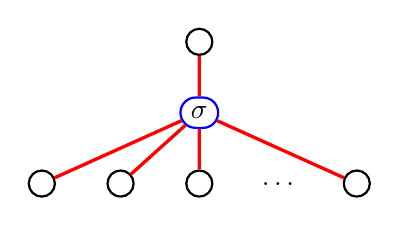
\begin{tikzpicture}
\begin{scope}[every node/.style={circle,thick,draw}]
    \node (A1) at (0,0) {};
    \node (A2) at (1,0) {};
    \node (A3) at (2,0) {};
    \node (A5) at (4,0) {};
    \node (C) at (2,1.8) {};
\end{scope}
\begin{scope}[every node/.style={rounded rectangle,thick,draw=blue}]
    \node (B) at (2,.9) {$\sigma$};
\end{scope}
\node (T) at (3,0) {$\ldots$};
\begin{scope}[>={Stealth[black]},
              every edge/.style={draw=red,very thick}]
    \path [-] (A1) edge node {}(B);
    \path [-] (A2) edge node {}(B);
    \path [-] (A3) edge node {}(B);
    \path [-] (A5) edge node {}(B);
    \path [-] (B) edge node {}(C);
\end{scope}
\end{tikzpicture}
\end{document}  

%
%
%
%
%
%
%
%
%
%
%
%
%
%
%
%
%
%
%
%
%
%
%
%
%
%
%
%
















